\documentclass[fleqn,usenatbib]{mnras}

% MNRAS is set in Times font. If you don't have this installed (most LaTeX
% installations will be fine) or prefer the old Computer Modern fonts, comment
% out the following line
\usepackage{newtxtext,newtxmath}
\usepackage{times}
% Depending on your LaTeX fonts installation, you might get better results with one of these:
% \usepackage{mathptmx}
% \usepackage{txfonts}

% Use vector fonts, so it zooms properly in on-screen viewing software
% Don't change these lines unless you know what you are doing
\usepackage[T1]{fontenc}
\usepackage{ae,aecompl}

%%%%% AUTHORS - PLACE YOUR OWN PACKAGES HERE %%%%%
%\usepackage{epsf}
\usepackage{color}
\usepackage{graphicx}
\usepackage{amsmath}	% Advanced maths commands
\usepackage{amssymb}	% Extra maths symbols
\usepackage{natbib}
%\usepackage[colorlinks,urlcolor=blue,citecolor=blue,linkcolor=blue]{hyperref}
\usepackage{multirow}
\usepackage{etoolbox}

%%%%% AUTHORS - PLACE YOUR OWN COMMANDS HERE %%%%%
%%% Fields %%%
\newcommand{\hdf}{HDF-N}
\newcommand{\hdfn}{HDF-N}
\newcommand{\hdfs}{HDF-S}
\newcommand{\cdfs}{CDF-S}

%%% Telescopes %%%
\newcommand{\hst}{\textit{HST}}
\newcommand{\iras}{\textit{IRAS}}
\newcommand{\iso}{\textit{ISO}}
\newcommand{\spitzer}{\textit{Spitzer}}
\newcommand{\sirtf}{\textit{Spitzer}}
\newcommand{\chandra}{\textit{Chandra}}

%%% Filters %%%
\newcommand{\wfu}{\hbox{$\mathrm{U}_{300}$}}
\newcommand{\wfb}{\hbox{$\mathrm{B}_{450}$}}
\newcommand{\wfv}{\hbox{$\mathrm{V}_{606}$}}
\newcommand{\wfi}{\hbox{$\mathrm{I}_{814}$}}
\newcommand{\acsb}{\hbox{$\mathrm{B}_{435}$}}
\newcommand{\acsv}{\hbox{$\mathrm{V}_{606}$}}
\newcommand{\acsi}{\hbox{$i_{775}$}}
\newcommand{\acsz}{\hbox{$z_{850}$}}
\newcommand{\nicj}{\hbox{$\mathrm{J}_{110}$}}
\newcommand{\nich}{\hbox{$\mathrm{H}_{160}$}}
\newcommand{\wfcy}{\hbox{$\mathrm{Y}_{105}$}}
\newcommand{\wfcj}{\hbox{$\mathrm{J}_{125}$}}
%\newcommand{\wfcj}{\hbox{$J_{110}$}}
\newcommand{\wfch}{\hbox{$\mathrm{H}_{160}$}}
\newcommand{\sdssu}{\hbox{$u$}}
\newcommand{\sdssg}{\hbox{$g$}}
\newcommand{\sdssr}{\hbox{$r$}}
\newcommand{\sdssi}{\hbox{$i$}}
\newcommand{\sdssz}{\hbox{$z$}}
\newcommand{\mone}{\hbox{$[3.6]$}}
\newcommand{\mtwo}{\hbox{$[4.5]$}}
\newcommand{\mthree}{\hbox{$[5.8]$}}
\newcommand{\mfour}{\hbox{$[8.0]$}}
%\newcommand{\mone}{\hbox{$[3.6\mu\mathrm{m}]$}}
%\newcommand{\mtwo}{\hbox{$[4.5\mu\mathrm{m}]$}}
%\newcommand{\mthree}{\hbox{$[5.8\mu\mathrm{m}]$}}
%\newcommand{\mfour}{\hbox{$[8.0\mu\mathrm{m}]$}}

%%% Astronomy Abreviations %%%
\newcommand{\mstar}{\hbox{$\mathrm{M}^\ast$}}
\newcommand{\lstar}{\hbox{$L^\ast$}}
\newcommand{\Msol}{\hbox{$\mathrm{M}_\odot$}}
\newcommand{\msol}{\hbox{$\mathrm{M}_\odot$}}
\newcommand{\Zsol}{\hbox{$Z_\odot$}}
\newcommand{\zsol}{\hbox{$Z_\odot$}}
\newcommand{\Lsol}{\hbox{$L_\odot$}}
\newcommand{\lsol}{\hbox{$L_\odot$}}
\newcommand{\lir}{\hbox{$L_{\mathrm{IR}}$}}
\newcommand{\zph}{\hbox{$z_\mathrm{ph}$}}
\newcommand{\zphot}{\hbox{$z_\mathrm{ph}$}}
\newcommand{\lbol}{\hbox{$L_\mathrm{bol}$}}
\newcommand{\snr}{\hbox{$\mathrm{S/N}$}}
\newcommand{\reff}{\hbox{$r_\mathrm{eff}$}}
\newcommand{\ks}{\hbox{$K_s$}}
\newcommand{\AAA}{\hbox{\AA}}

%%% Spectrum Lines %%%
\newcommand{\lya}{ Ly$\alpha \;$}
\newcommand{\lyb}{Lyman~$\beta$}
\newcommand{\hb}{\hbox{H$\beta$}}
\newcommand{\ha}{\hbox{H$\alpha$}}
\newcommand{\paa}{\hbox{Pa$\alpha$}}

%%% Units %%%
\newcommand{\kms}{\hbox{km~s$^{-1}$}}
\newcommand{\cms}{\hbox{cm~s$^{-1}$}}
\newcommand{\mpc}{\hbox{Mpc$^{-1}$}}
\newcommand{\mpcsq}{\hbox{Mpc$^{-2}$}}
\newcommand{\mpccu}{\hbox{Mpc$^{-3}$}}
\newcommand{\cnts}{\hbox{cnt~s$^{-1}$}} 
\newcommand{\cmsq}{\hbox{cm$^{-2}$}}
\newcommand{\cmcu}{\hbox{cm$^{-3}$}}
\newcommand{\ergscm}{\hbox{erg~s$^{-1}$~cm$^{-2}$}}
\newcommand{\uJy}{\hbox{$\mu$Jy}}
\newcommand{\ujy}{\hbox{$\mu$Jy}}
\newcommand{\degree}{\hbox{$^\circ$}}
\newcommand{\degsq}{\hbox{degree$^2$}}
\newcommand{\arcminsq}{\hbox{arcmin$^2$}}
\newcommand{\um}{\hbox{$\mu$m}}

%%% Math %%%
\newcommand{\lsim}{\lesssim}
\newcommand{\gsim}{\gtrsim}
\newcommand{\mathS}{\hbox{$\mathcal{S}$}}
\newcommand{\mathR}{\hbox{$\mathcal{R}$}}
\newcommand{\mathM}{\hbox{$\mathcal{M}$}}
\newcommand{\mcal}{\hbox{$\mathcal{M}$}}
\newcommand{\rcal}{\hbox{$\mathcal{R}$}}
\newcommand{\scal}{\hbox{$\mathcal{S}$}}
\newcommand{\infinity}{\hbox{$\infty$}}
\newcommand{\err}[2]{$^{+#2}_{-#1}$}

%%% General %%%
\newcommand{\etal}{et al.}
\newcommand{\eg}{e.g.}
\newcommand{\ie}{i.e.}
\newcommand{\cf}{cf.}
% \newcommand{\ion}[2]{\hbox{#1$\;${\small\rm{#2}}}}
\newcommand{\mybullet}{\noindent$\bullet$}
\newcommand{\uit}{\textit{UIT}}
\newcommand{\nd}{...}
%\newcommand{\cmodel}{\hbox{\tt cmodel}}
%\newcommand{\bs}{\hbox{$\!\!\!\!$}}
\newcommand{\todo}[1]{{\tt #1}}
\newcommand{\citeeg}[1]{(\eg, \citealt{#1})}
\newcommand{\ignore}[1]{}

%%% Extra %%% 
% \newcommand{\farcm}{\mbox{\ensuremath{.\mkern-4mu^\prime}}}%fractional arcminute symbol 0.'0
% \newcommand{\farcs}{\mbox{\ensuremath{.\!\!^{\prime\prime}}}}%fractional arcsecond symbol: 0.''0
% \newcommand{\fdg}{\mbox{\ensuremath{.\!\!^\circ}}}%fractional degree symbol:     0.°0
\newcommand{\arcdeg}{\ensuremath{^{\circ}}}%                    % degree symbol:  °
% \newcommand{\sun}{\ensuremath{\odot}}%                          % sun symbol
% \newcommand{\apj}{ApJ}%                                         % Journal abbreviations
% \newcommand{\apjs}{ApJS}
% \newcommand{\apjl}{ApJL}
% \newcommand{\aap}{A{\&}A}
% \newcommand{\aaps}{A{\&}AS}
% \newcommand{\mnras}{MNRAS}
% \newcommand{\aj}{AJ}
% \newcommand{\araa}{ARAA}
% \newcommand{\pasp}{PASP}
\newcommand{\Teff}{\ensuremath{T_{\mathrm{eff}}}}%              % T_eff
\newcommand{\logg}{\ensuremath{\log g}}%                        % log g
\newcommand{\bv}{\ensuremath{B\!-\!V}}%                         % B-V
\newcommand{\ub}{\ensuremath{U\!-\!B}}%                         % U-B
\newcommand{\vr}{\ensuremath{V\!-\!R}}%                         % V-R
\newcommand{\ur}{\ensuremath{U\!-\!R}}%                         % U-R

\newcommand{\editorial}[1]{\textcolor{red}{#1}}
\DeclareRobustCommand{\ion}[2]{%
\relax\ifmmode
\ifx\testbx\f@series
{\mathbf{#1\,\mathsc{#2}}}\else
{\mathrm{#1\,\mathsc{#2}}}\fi
\else\textup{#1\,{\mdseries\textsc{#2}}}%
\fi}
\newcommand{\multic}[2]{\multicolumn{#1}{c}{#2}}
\newcommand{\rottext}[2]{\multirow{#1}{*}{\rotatebox[origin=c]{90}{#2}}}

%%%%%%%%%%%%%%%%%%% TITLE PAGE %%%%%%%%%%%%%%%%%%%
\title[Short Title]{Cluster Dynamics with HETDEX at z < 0.5 - I: Simulated Performance, Mass Distribution and Limits}

% The list of authors, and the short list which is used in the headers.
% If you need two or more lines of authors, add an extra line using \newauthor
\author[S. Boada et al.]
{\parbox{\textwidth}{Steven Boada,$^{1}$\thanks{E-mail: boada@physics.tamu.edu}
C.~Papovich,$^{1}$
R.~Wechsler,$^{2,3}$
T. S.~Li,$^{1}$
K.~Gebhardt,$^{5}$
E.~Rozo,$^{2,4}$
E. S.~Rykoff$^{2}$}\vspace{0.4cm}\
\\
\parbox{\textwidth}{$^{1}$George P.\ and Cynthia Woods Mitchell Institute for Fundamental Physics and Astronomy, and Department of Physics and Astronomy, Texas A\&M University, College Station, TX, 77843-4242, USA\\
$^{2}$Kavli Institute for Particle Astrophysics and Cosmology, Department of Physics, Stanford University, Stanford, CA 94305, USA\\
$^{3}$Department of Particle Physics and Astrophysics, SLAC National Accelerator Laboratory, Menlo Park, CA 94025, USA\\
$^{4}$Department of Physics, University of Arizona, Tucson, AZ 85721, USA\\
$^{5}$Department of Astronomy, The University of Texas at Austin, Austin, TX 78712, USA}}

% These dates will be filled out by the publisher
\date{Accepted XXX. Received YYY; in original form ZZZ}

% Enter the current year, for the copyright statements etc.
\pubyear{2016}

% Don't change these lines
\begin{document}
\label{firstpage}
\pagerange{\pageref{firstpage}--\pageref{lastpage}}
\maketitle

\begin{abstract}
\noindent
The study of clusters of galaxies has been argued to be a very effective way to measure cosmological parameters, including measuring dark energy and testing models of gravity. The Hobby Eberly Telescope Dark Energy Experiment (HETDEX) will observe many hundreds of square degrees, covering a large sample of galaxy clusters out to $z = 0.5$ based on their optical spectra ($3500-5500\AAA$). The spectra will provide important measures of the clusters dynamics and may enable constraints on cosmological parameters, but only if the measurements provide accurate estimates of the total cluster masses. We have carried out a study to investigate the ability of HETDEX to recover accurate galaxy cluster masses over a wide range of masses and redshifts. We used a detailed mock galaxy catalog and present mock observations of two different scenarios: (1) We targeted individual galaxy clusters to investigate the recovery of parameters with such observations. (2) We created and evaluated a HETDEX-like selection "function'' of galaxies over a similarly sized portion of the sky and use well adopted techniques to recover the dynamical properties, such as velocity dispersion and mass, and benchmark these against observations with perfect knowledge. Using both observing strategies, we produce cluster mass probability density functions $P(X|M,z)$, which can be used to determine the probability that a galaxy cluster of given mass (M), located at redshift ($z$) determined using observable parameter (X). \editorial{This sentence will summarize how well HETDEX will do, and how that might be improved with targeted observations.}
\end{abstract}

\section{INTRODUCTION}
\editorial{The introduction is now much longer because I talked about the cons to the different cluster mass recovery methods. I don't much care for really long introductions, so if there is anything that could by cut to shorten it, I would be ok.}
Our ability to perform precision cosmology with clusters of galaxies has reached a critical turning point. The widely accepted $\Lambda$CDM model of cosmology makes explicit predictions about the number and masses of galaxy clusters throughout the universe. However, connecting these predictions to a set of, sufficiently large in size, observed clusters remains a principal problem. Specifically, the largest threat to modern, precision, cluster cosmology is not the identification of large numbers of clusters (the total number of clusters known is only going up) but the accurate recovery of galaxy cluster mass \citeeg{Sehgal2011,Plank2014, Bocquet2015}.

As mass is not a direct observable, a lot of work is underway to characterize galaxy cluster masses with an observable feature of galaxy clusters. The goal is to constrain, as best possible, $P(M|x)$ the probability ($P$) that a galaxy cluster of given mass ($M$), located at redshift ($z$) determined using observable parameter ($X$). Generally, cluster mass calibrations fall into two distinct camps, simulation based and direct or statistical calibration.

One could use various simulations to attempt to calibrate this observable--mass relation \citeeg{Vanderlinde2010, Sehgal2011}. However, the primary challenge to this method is the incomplete understanding of the baryonic physics which take place in galaxy cluster environments. While there have been (and continue to be) many improvements in the accuracy and power of simulations it is doubtful that in the coming years they will reach the accuracy level required to the point where the observable--mass relation is dominated only by statistics \citep{Weinberg2013}. 
 
The second broad camp is the direct calibration of cluster masses. This recipe has two distinct but not always independent tracks. The ``direct'' method uses the direct observations of a small set of clusters and then uses known mass estimators, X-ray temperatures and luminosities \citeeg{Mantz2010, Rykoff2014}, cosmic microwave background (CMB) observations \citeeg{Vanderlinde2010, Sehgal2011}, optical richness \citeeg{Abell1958, Rykoff2012} or weak lensing (WL) \citeeg{Rozo2010} as examples, which provide a ``true'' mass. This directly calibrates the observable--mass relation which is then applied to a much larger sample. The complications lie in that the ``true'' masses are in fact estimations, and the methods used to recover these masses are subject to their own limitations. X-ray hydrostatic estimations assume hydrostatic equilibrium \citeeg{Mantz2015} which may only be valid for a very small number and range of cluster masses. The Sunyaev--Zel'dovich Effect (SZE; \citealt{Sunyaev1972}), which uses the up--scattering of CMB photons to estimate cluster masses, provides accurate estimations of mass, but the ability to detect low mass galaxy clusters is currently limited by technology \citeeg{Carlstrom2002a}. WL estimates are, in principle, correct in the mean, but they suffer from signal-to-noise requirements, limiting their usefulness in low mass clusters, and potentially suffer from line-of-sight effects as the effect is sensitive to all mass along the line of sight. Virial mass estimators which determine the cluster mass based on the motions of the member galaxies \citeeg{Ruel2014, Sifon2015} are promising in that it is a direct measurement of the depth of clusters potential well, but suffers from systematics due to cluster formation physics which disrupts the velocity field.
 
The statistical method of determining galaxy cluster mass relies not on direct measurements of individual clusters but the calibration of observables for the entire sample which correlate with cluster mass. One example is the spatial clustering of the galaxy clusters themselves. See \cite{Weinberg2013} for a comprehensive review. In practice, it will be a combination of the three methods touched on that will provide the most reliable determination of cluster masses.

Massive surveys, both on going and planned, are revolutionizing cluster cosmology using a large range of wavelengths. The South Pole Telescope (SPT; \citealt{Carlstrom2011}) and the Atacama Cosmology Telescope (ACT; \citealt{Swetz2011}) are discovering many clusters through the SZE. Optically, the on going The Dark Energy Survey (DES; \citealt{DES2005}) and planned Large Synoptic Survey Telescope (LSST; \citealt{LSST2012}) will identify many thousands of clusters to much lower masses than is possible with SZE measurements. However, regardless of the discovery method used, spectroscopic followup is needed to further constrain $P(X|M,z)$. But as the cluster dataset grows to many tens of thousands of clusters individual followup becomes increasingly impractical. Therefore, large spectroscopic surveys are needed to more fully constrain the observable--mass relation of clusters.

The Hobby Eberly Telescope Dark Energy eXperiment (HETDEX; \citealt{Hill2008}) is a trailblazing effort to observe high-redshift large scale structures using cutting edge wide-field integral field unit (IFU) spectrographs. Designed to probe the evolution of the dark energy equation of state etched onto high redshift ($z>2$) galaxies by the Baryon Acoustic Oscillations \citep{Eisenstein2005} in the first moments of the universe, the survey will observe two fields for a total of 420 \degsq\ from two fields (300 \degsq, Spring field and 120 \degsq, Fall field). Tuned to find \lya\ emitting (LAE) galaxies at $1.9<z<3.5$, HETDEX expects to find 800,000 LAEs, and more than one million [\ion{O}{ii}] emitting galaxies at $z<0.5$ masquerading as high-redshift galaxies \citep{Acquaviva2014}. 

While a large portion of the $\sim10^6$ interloping [\ion{O}{ii}] galaxies will be field (not associated with a bound structure) galaxies, the large area covered by HETDEX is expected to contain as many as 50 Virgo-sized ($M_{dyn}\sim 10^{15}$ \msol) clusters at $z<0.5$ (\editorial{talk to casey about how I calculated this number}). The near-complete spectroscopic coverage allows an unprecedentedly detailed look at a very large number of clusters ranging from group scales to the very massive. In addition to the recovery of accurate dynamical masses, detailed investigations of the of dynamical state of the clusters is possible. 

Connecting the dynamical properties derived from spectroscopy to the properties inferred from other studies insures the greatest impact on future work. HETDEX overlaps with the Sloan Digital Sky Survey (SDSS; \citealt{Blanton2001a}), SDSS stripe 82 \citep{Annis2014}, the Dark Energy Survey (DES; \citealt{DES2005}), and the upcoming DECam/IRAC Galaxy Environment Survey (DIRGES; PI: Papovich, C. Papovich \etal\ in preparation), the The \emph{Spitzer}/HETDEX Exploratory Large-Area Survey (SHELA; Papovich \etal\ 2016, ApJS, submitted), and The \emph{Spitzer} IRAC Equatorial Survey (SpIES; Timlin \etal\ 2016, ApJ, submitted). While the potential dataset is very rich, two large issues remain.

It is unclear how a blind spectroscopic survey with an IFU will effect the recovery of galaxy cluster dynamical properties. Unlike many previous large cluster surveys \citeeg{Milvang-Jensen2008, Robotham2011, Sifon2015} which use multi-object spectrographs, the Visible Integral-Field Replicable Unit Spectrograph (VIRUS; \citealt{Hill2012}) used by HETDEX samples the sky unevenly which could excluded member galaxies which would otherwise be included. Secondly, it is not straightforward to use spectroscopic redshifts predominately from emission-line galaxies to interpret the kinematic and dynamical states of the clusters.

\editorial{The wording here needs to be updated when we settle on the verbage for everything else.} This work plans to address these concerns in the following ways. We use simulated observations which target individual galaxy clusters to investigate the recovery of parameters with such observations. Secondly, we create and evaluate a HETDEX like selection ``function'' of galaxies over a similarly large portion of the sky and use well adopted techniques to recover the dynamical properties, such as velocity dispersion and mass. Each observation strategy will further be constrained with ``ideal'' and ``realistic'' knowledge. Ideal knowledge assumes that we know which individual galaxy is assigned to which cluster. With realistic knowledge this is unknown and must be determined prior to the estimation of the cluster properties. Both of these strategies will better allow future work to predict the number and types of galaxy clusters which should be observed with VIRUS during both the HETDEX survey portion and through targeted follow up observations.

We begin in Section \ref{sec:Data} by giving an overview of what data is used, how it is created, and how we make our ``observations.'' Details about the determination of cluster parameters, velocity dispersion, total mass, etc., are discussed in Section \ref{sec:recovery}. Next, we present the results of our study in Section \ref{sec:results} and discuss their implications in Section \ref{sec:discussion}. Finally we summarize our findings in Section \ref{sec:summary}.

Throughout this paper, we adopt the following cosmological model: $\Omega_\Lambda = 0.714$,
$\Omega_M = 0.286$, $\sigma_8 = 0.82$ and $H_0= 70$ \kms \mpc (taken from the Buzzard catalogs; see below), assume a Chabrier initial mass function (IMF; \citealt{Chabrier2003}), and use AB magnitudes \citep{Oke1974}.

\section{Data and Mock Observations}\label{sec:Data}
In this section, we describe the data products and the techniques used to replicate the HETDEX survey. We use the information from a large mock galaxy catalog supplemented by galaxies from the SDSS to create a realistic ``sky'' and ``observe'' it with a HETDEX-like observing strategy.

\subsection{The ``Buzzard'' Catalogs}
\begin{figure*} 
	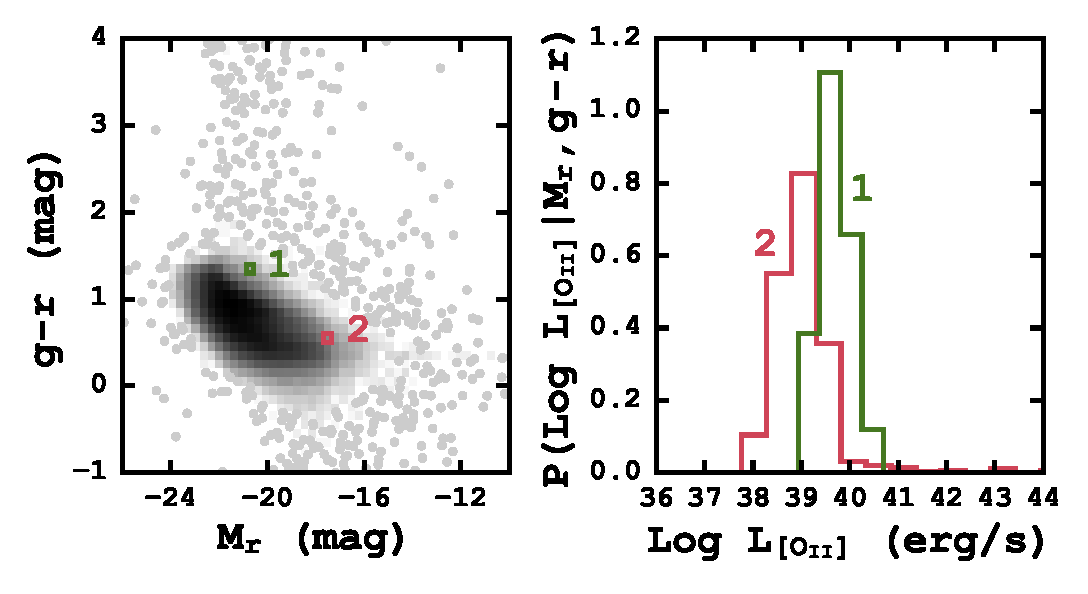
\includegraphics[width=\textwidth]{figures/oii_sdss.pdf} 
	\caption{\textit{Left}: CMD of 503113 $z<0.2$ galaxies take from the SDSS DR12 where the shading scales with the density of points. The two colored boxes show regions containing potential catalog galaxies. \textit{Right}: Probability histograms of the Log [\ion{O}{ii}] luminosity for the SDSS galaxies located in the two highlighted regions on the right. New [\ion{O}{ii}] luminosity (and subsequently fluxes) are assigned to catalog galaxies from slice sampling the probability histogram. See the text for a full description of the process.} \label{fig: oii sdss} 
\end{figure*}

The ``Buzzard'' mock galaxy catalogs (R. Wechsler et al., private communication) cover 375.68 \degsq\ between $4^h< RA < 6^h$ and $-61\degree < DEC < -41\degree$ and are derived from a combination of Sub-halo Abundance Matching (ShAM) and ADDSEDs (Adding Density Dependent Spectral Energy Distributions) tied to an in house n-body cosmological simulation. A brief description of the catalog creation is described as follows. The initial conditions are generated with a second-order Lagrangian perturbation theory using {\tt 2LPTic} \citep{Crocce2006}. Dark matter (DM) n-body simulations are run using {\tt LGadget-2} (a version of {\tt Gadget-2}; \citealt{Springel2005}). The DM halos are identified using the {\tt ROCKSTAR} halo finder \citep{Behroozi2013} which also calculates halo masses and other various parameters. 

Galaxy $M_r$ luminosities are added to the velocity peaks using ShAM \citep{Reddick2013}, and ADDSEDs (Adding Density Dependent Spectral Energy Distributions) assign luminosities in the other bands. A $M_r$-density-SED relation is created using a SDSS training set, and for each mock galaxy the SED of a randomly selected training set galaxy which has a similar $M_r$ and density is assigned. The result is a 398.49 sq. degree mock catalog occupying a $4^h \leq RA \leq 6^h$ and $-61\degree < DEC < -41\degree$ portion of the sky. It contains 238 million galaxies with \sdssr\ mag $< 29$ and $z \leq 8.7$.

The catalog information, used in this study, is broken into two large portions. The ``truth'' files contain the characteristics of each individual galaxies, such as right ascension (RA), declination (DEC), redshift ($z$), observed and rest-frame magnitudes, and many others. The ``halo'' files contain information for individual halos, to which many individual galaxies may belong. This includes five estimations of dynamical mass, RA, DEC, z, three dimensional velocity dispersion, and many others. However, the catalogs do not include information for emission lines. We supplement the catalogs by generating this information; the process is described in Section~\ref{sec: oii luminosity}.

% \begin{figure}
% 	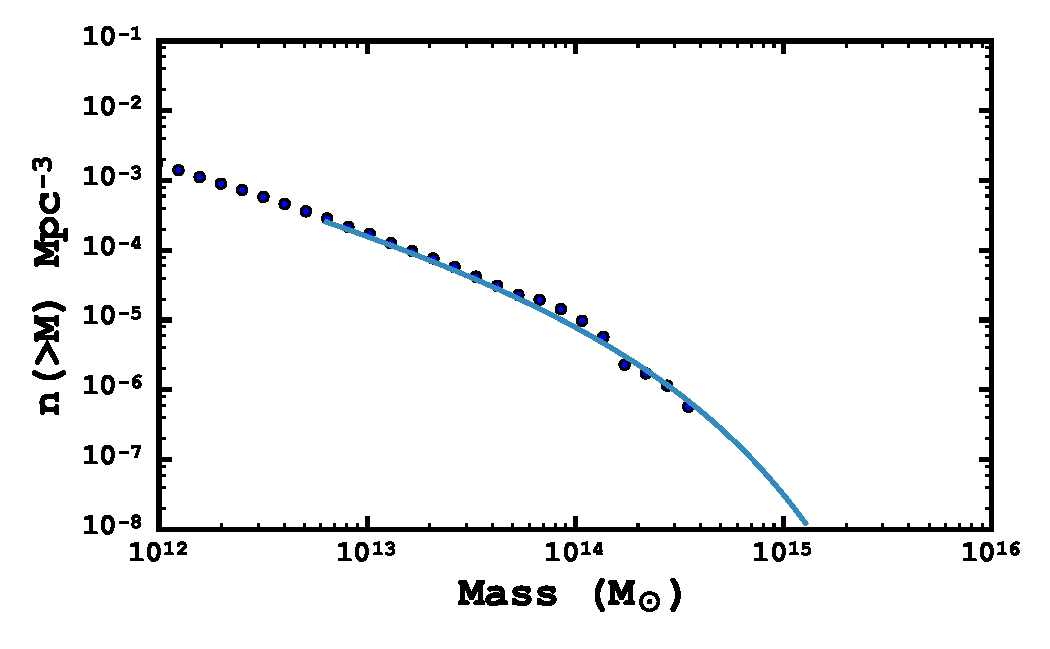
\includegraphics[width=\columnwidth]{figures/hmf.pdf}
% 	\caption{The cumulative MF (from \citealt{Tinker2008}) of halos above $M_{200c}$ at $z=0.1$}
% 	\label{fig: hmf}
% \end{figure}

We investigate the accuracy of the halo mass distribution by comparing the cumulative number density of halos above a mass ($M_{200c}$) threshold to the halo mass function (HMF) of \cite{Tinker2008}. We calculate the HMF is calculated at central redshifts of 0.1, 0.2, and 0.4 using {\tt HMFcalc} \citep{Murray2013} and compared to galaxies in a redshift window of $\Delta z\pm0.01$. We find a very good agreement between the predicted HMF and the observed distribution of clusters. \editorial{Could show a figure comparing the Buzzard catalog to a plot of the HMF for a couple of redshifts. Might be helpful, might not matter.}

\subsection{ {\rm[\ion{O}{ii}]} Luminosity}\label{sec: oii luminosity}
The Buzzard ``truth'' catalog does not provide [\ion{O}{ii}] luminosities so we must assign them empirically. We use 503113 galaxies from the SDSS Data Release 12 \citep{Alam2015} from $z = 0.05 - 0.2$, which are selected with no redshift warning, and place each galaxy on a color-magnitude diagram (CMD) of $M_r$ and $g-r$; see the left panel of Figure \ref{fig: oii sdss}.

To assign an [\ion{O}{ii}] luminosity to each galaxy in our catalog we place the catalog galaxies on the same CMD and select all SDSS galaxies in a small 2D ($M_r$, $g-r$) bin around the galaxy. We extract all of the SDSS galaxies inside that bin and create a histogram of their [\ion{O}{ii}] luminosities. Using a slice sampling technique \citep{Neal1997} we assign the catalog galaxy an [\ion{O}{ii}] luminosity based on the distribution of SDSS galaxies extracted. For catalog galaxies which are placed on the CMD near no, or very few ($1\leq n<10$) galaxies we assign it zero [\ion{O}{ii}] luminosity or the mean luminosity, respectively. For the galaxies in the Buzzard catalog, 1.3\% of the galaxies brighter than $\sdssg = 22$ mag (HETDEX's detection limit) have exactly zero [\ion{O}{ii}] luminosity. Of the 1.3\%, only 3.3\% (0.05\% of all galaxies) have $g-r < 1.5$ suggesting the galaxies which are assigned zero [\ion{O}{ii}] luminosity are not significantly biasing our simulations.

The right panel of Figure~\ref{fig: oii sdss} shows the CMD of all SDSS galaxies. Two potential catalog galaxies are also placed on the CMD ($M_r, g-r = -17.7,~0.49$ and $M_r, g-r = -21.4,~1.24$) and indicated by the two colored boxes. The histograms show in the Figure's right panel show the probability density histograms of the Log [\ion{O}{ii}] luminosity for the SDSS galaxies in the 2D bin around the individual catalog galaxies. We sample the distribution and assign each catalog galaxy an [\ion{O}{ii}] luminosity which is then converted into a flux. \editorial{We could add a plot like the corner plot to show the multi-dimensionality of this process.}

\subsection{Mock Observations}\label{sec: observations}
\begin{figure} 
	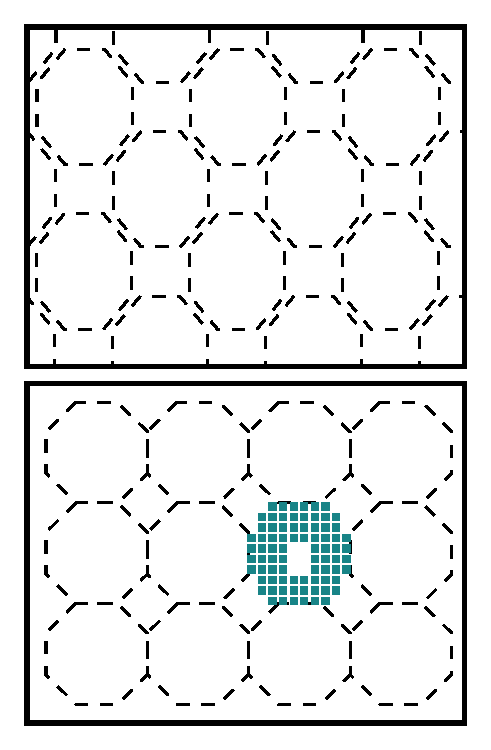
\includegraphics[width=\columnwidth]{figures/pointings.pdf} 
	\caption{Representative observation tiling scheme for the HETDEX $16' \times 16'$ pointings. Each colored square is a single VIRUS IFU and the dashed octagons approximate the size of a single observation. See the text for more details.} \label{fig: ifu layout} 
\end{figure}

Tentatively slated to start in the spring of 2016, HETDEX will perform blind spectroscopy (R $\sim$ 750 in $3500 - 5500~\AAA$) over two fields along the celestial equator. The 300 \degsq, spring field and 120 \degsq, fall field will have no preselected targets. Using VIRUS on the 10-m Hobby-Eberly Telescope (HET; \citealt{Ramsey1998}) the completed survey is expected to have an overall fill-factor of 1/4.5, meaning that the entire area could be covered with 4.5 dithers of the entire survey. 

Each mask is created to accurately reproduce the HETDEX IFU pattern, see Figure~\ref{fig: ifu layout}. The pattern consists of 78 IFUs, which are comprised of 448 optical fibers subtending a $50'' \times 50''$ region on the sky \citep{Kelz2014}. The inter-IFU spacing is also $50''$ spanning a total area of $16'\times 16'$ on the sky. 

The individual IFUs have a fill-factor of 1/3, which will be completely filled with three dithers of the telescope at each pointing. This means that when selecting galaxies from the Buzzard catalog we assume an observation for all galaxies laying within a colored, IFU square in Figure~\ref{fig: ifu layout}. Galaxies which lie between the IFUs are missed, as well as the galaxies which lie between the pointings, as there is no overlap between one pointing and the next. To cover the 375.67 \degsq\ field of the Buzzard catalog we require 5370 pointings where 0.015 \degsq\ of each pointing is covered by an IFU. The total area of the sky covered by an IFU is 80.80 \degsq\ which gives a filling factor of 1/4.65 slight decreased from the expected filling factor of 1/4.5.

The spectral coverage allows for the detection of [\ion{O}{ii}] ($\lambda\lambda 3727,3729~\AAA$ doublet) emitters to $z\sim 0.5$ and Ca H ($\lambda 3968.5~\AAA$) and K ($\lambda 3933.7~\AAA$) absorption features to $z\sim 0.4$. HETDEX is expected to detect sources with continuum brighter than $\sdssg=22$ mag, and emission line strengths above $3.5\times10^{-17}$ \ergscm.

In this work we consider two separate observing strategies, targeted and survey-like. The targeted observations use ``direct'' observations where each cluster is targeted individual, and every cluster member galaxy is assumed to be observed. The survey observations mimic the HETDEX observation pattern across the sky, where no cluster is directly targeted and not all cluster member galaxies are observed. Both of these observations have HETDEX-like galaxy detection thresholds, for comparison we also include a set of targeted observations with ``perfect'' knowledge. ``Perfect'' observations assume no detection threshold, if a cluster member galaxy is observed, it is also detected. This provides an important best-case scenario, and differs from the true cluster properties because the recovered cluster properties are still calculated. These observations provide three levels of quality with ``perfect knowledge'' being the highest and survey being the lowest.

\section{Recovery of Parameters}\label{sec:recovery}
 In the following sections, we outline the methods we use to derive the dynamical properties of the galaxy clusters in our sample. This is not meant to be an exhaustive study of the different methods used to recover these parameters. The following is, in many cases, a subset of the available methods to derive any single parameter. The specific choice of method may improve or diminish the accuracy of the recovered parameter, but the methods chosen were to facilitate comparison with observational studies. 

\subsection{Cluster Redshift}
The accurate determination of the cluster redshift ($z_c$) is crucial to the reliability of all following measurements. An incorrect cluster redshift introduces errors into the measured line-of-sight velocity (LOSV) and corresponding dispersion, which, in turn, contributes to errors associated with dynamical mass and radius. 

In simple terms, the cluster redshift is the mean of the redshifts of all galaxies associated with the cluster. However, because the standard mean can be quite sensitive to outliers or otherwise contaminated data, we require a more resistant statistic, and turn to the biweight location estimator \citep{Beers1990} which provides improved performance. 

\subsection{Line-of-Sight Velocity Dispersion}\label{sec: LOSVD}
We first calculate the line-of-sight velocity (LOSV) to each galaxy, where
\begin{equation}
	LOSV = c\frac{z - z_c}{1+z_c}
\end{equation}
and $c$ is the speed of light in \kms, $z$ is the redshift of the individual galaxy, and $z_c$ is the overall cluster redshift described in the previous section.

The line-of-sight velocity dispersion (LOSVD) is calculated using a method of maximum likelihood following \cite{Walker2006}. We maximize the probability function 
\begin{equation}
  \label{eq: jointGaussian}
p(\{v_1, ..., v_N\})=\displaystyle\prod_{i=1}^{N}\frac{1}{\sqrt{2\pi(\sigma_i^2+\sigma_p^2)}}\exp\biggl[-\frac{1}{2}\frac{(v_i-\langle u \rangle)^2}{(\sigma_i^2+\sigma_p^2)}\biggr]
\end{equation}
where $\sigma_p$, $\langle\mu\rangle$, and $\sigma_i$ is the LOSVD, the average radial velocity and the error on the individual LOSVs respectively. Using a Monte Carlo Markov Chain (MCMC) sampler ({\tt emcee}\footnote{\url{http://dan.iel.fm/emcee/current/}}; \citealt{Foreman-Mackey2013}) which is based on affine-invariant ensemble sampler (see \citealt{Goodman2010} for details on affine-invariant samplers). We draw twenty thousand samples from the posterior probability distribution using simple priors, $\langle\mu\rangle$ lies between the maximum and minimum LOSV and $0< \sigma_p < 1400$ \kms. When the full distribution of LOSVDs are not used, the final LOSVD is quoted as the median value of the posterior probability distribution with 68\% error bars defined as the 16th and 84th percentiles of the same distribution.

In principle, a single statistic such as the biweight scale estimator or the gapper estimator (both from \citealt{Beers1990}) with many bootstrap resamplings could be used to construct a distribution of $\sigma_p$. In simple tests where the values of both $\sigma_p$ and $\langle\mu\rangle$ are known. The 68\% error bars derived from the MCMC method give slightly better results with the true LOSVD value bracketed by the error bars in $\sim68\%$ of the cases versus $\sim57\%$ with bootstrapping and a single statistic. In addition, we prefer the maximum likelihood method for its straight forward treatment of the errors in the LOSV measurements.

\subsection{Dynamical Mass}\label{sec: mass}
The relationship between the LOSVD and dynamical mass has been the focus of several studies \citeeg{Evrard2008, Saro2013, Sifon2013, VanderBurg2014}, and a best fitting relationship for the mass enclosed by $r_{200c}$ of the form
\begin{equation}\label{eq:power law}
	M_{200c} = \frac{10^{15}}{h(z)} \bigg{(}\frac{\sigma_{1D}}{A_{1D}} \bigg{)}^{1/\alpha} \Msol
\end{equation}
with $A_{1D} = 1177 \pm 4.2$ \kms\ (\citealt{Munari2013}; referred to as $\sigma_{15}$ in \citealt{Evrard2008} and other works), $\alpha = 1/3$, $h(z) = H(z)/100$, and $\sigma_{1D}$ is the LOSVD of the velocity tracers (dark matter particles, subhalos or galaxies). 

A growing body of work suggests that there is a significant difference in the observed LOSVD depending on the velocity tracers used. Specifically, while there is little difference between using galaxies and their host DM subhalos, there is a significant over estimation of the LOSVD when using galaxies/subhalos compared to DM particles \citep{Munari2013}. We follow other works \citeeg{Kirk2015, Sifon2015a} using the scaling relation, given in Equation~\ref{eq:power law} from \cite{Munari2013} to facilitate comparisons with other observational studies. 
% \editorial{This all needs to be stripped out and reworked.}
% The choice $A_{1D}$ and $\alpha$ varies between studies \citeeg{Munari2013, VanderBurg2014} and should be calibrated on a individual basis. To do this, we randomly select 47494, $z<0.5$ clusters composed of 36000 $10^{13}$, 6000 $10^{14}$ and two $10^{15}~\Msol$ halos. We perform a linear fit to the $\sigma_{1D}-M_{200}$ values allowing both $A_{1D}$ and $\alpha$ to vary. We find best fitting parameters of $A_{1D} = 1117.9~\kms$ and $\alpha = 0.3297$, both of which are very near the values from \cite{Evrard2008} of $A_{1D} = 1082.9 \pm 4.0~\kms$ and $\alpha = 0.3361$. Therefore, we chose to adopt the parameters from \cite{Evrard2008} to better facilitate with other simulations \citeeg{Old2014}, and observational studies \citeeg{Brodwin2010}.

\subsection{Dynamical Mass Corrections}
In this section we use two methods to predict the mass of a cluster based on other observables. Often the cluster mass is estimated based on a single observable, X-ray temperature, velocity dispersion, richness and others. Here we combine many observables to attempt to correct the mass inferred solely from the velocity dispersion. The first method is traditional probability based where we marginalize over a series of observables to find the most probable mass. The second is based on a machine learning (ML) algorithm which attempts to ``learn'' the relationship between the observables and the desired output, the mass. Both of these methods are examples of supervised learning algorithms where the relationship between the observable (known) parameters and the target parameter (the mass) are both known.

As with any predictive analysis it is important to test the model on data that the model has not seen before. In this section we take all of the observed clusters, our full sample, split them, and generate a training and testing set. The data is randomly split 70\% training and 30\% testing. We follow the ML convention and refer to the individual clusters in each set as a ``sample'', and the parameters associated with the cluster ($z$, LOSVD, mass, etc.) as ``features''.  

\subsubsection{Probability Based}\label{sec:probability method}
We begin with the training sample. After selecting the desired features $\vec{x} = \{\sigma, z, ...\}$ we make the joint probability between the true cluster mass (M) and $\vec{x}$. Because $\vec{x}$ can be multidimensional, we rely on the ``corner plot'' as an aid to visualize the relationship between all of the training features. Figure~\ref{fig: probability corner} shows all of the one (marginalized probability) and two (joint probability) dimensional projections of the posterior probability distributions of the features of the training data.

\begin{figure} 
	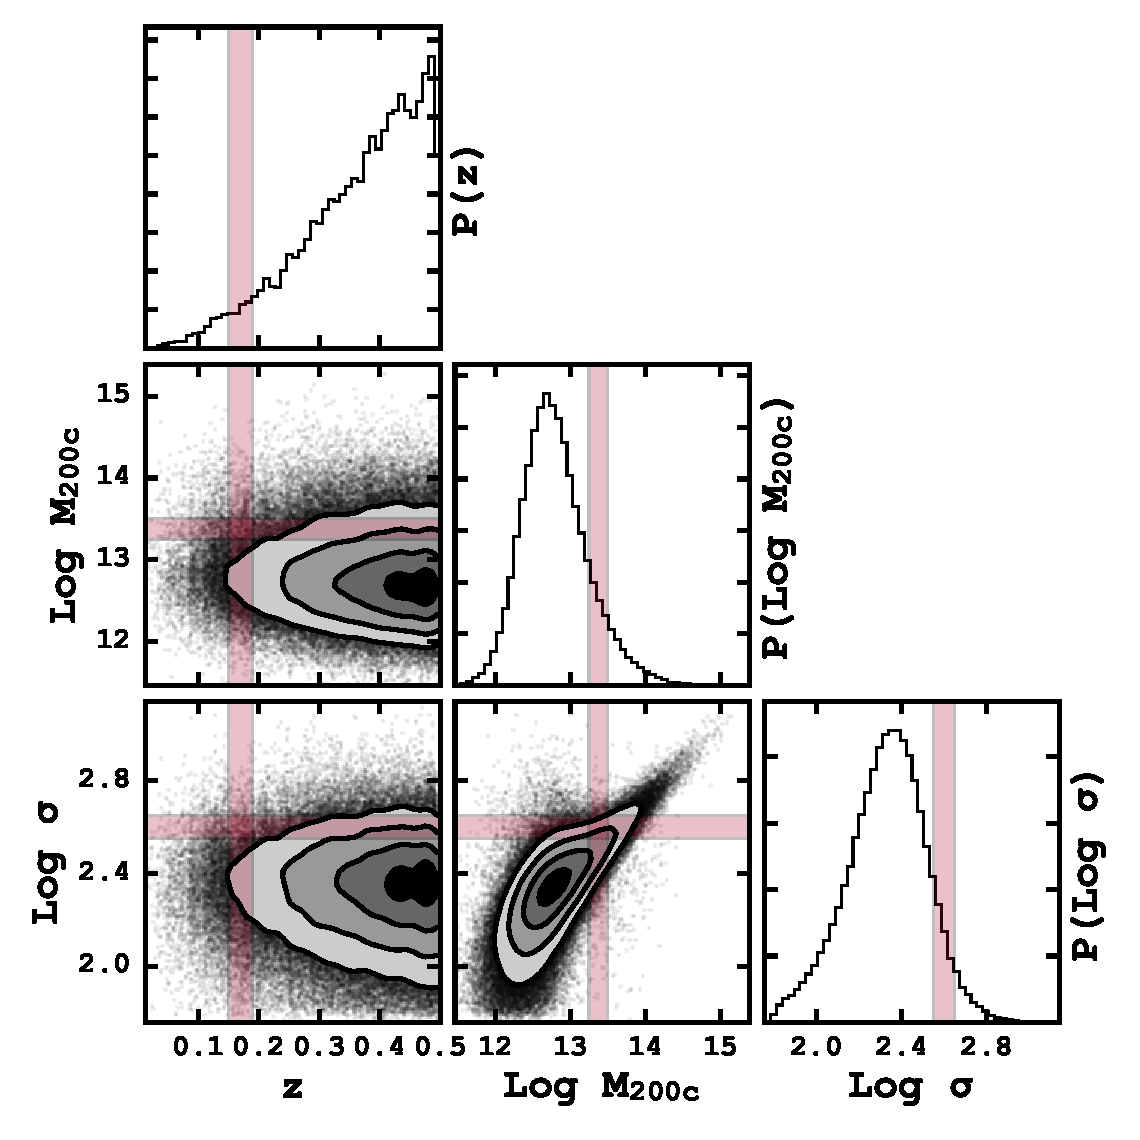
\includegraphics[width=\columnwidth]{figures/cornertest.pdf} 
	\caption{Corner plot of the \emph{training} data with features $\sigma$ and $z$. The corner plots shows all of the one and two dimensional posterior probability distributions used to determine the correct cluster mass. The colored rectangles, which have been enlarged for clarity, show the slices needed to create a conditional probability distribution of the mass, $P(M|\vec{x})$. See text for a complete description. } \label{fig: probability corner} 
\end{figure}

The conditional probability of the mass $P(M|\vec{x}= \{ x_1,x_2,...\})$ is determined by taking a slice through the joint probability distributions in bins centered on the desired value. The slices show by the colored bars in Figure~\ref{fig: probability corner} are centered on $\sigma = 400$ \kms and $z=0.17$. The distribution of mass contained in the three dimensional bin given by the intersection of these slices is $P(M|\vec{x} = \{ \sigma=400 \kms,z=0.17\})$.

\begin{figure*}
	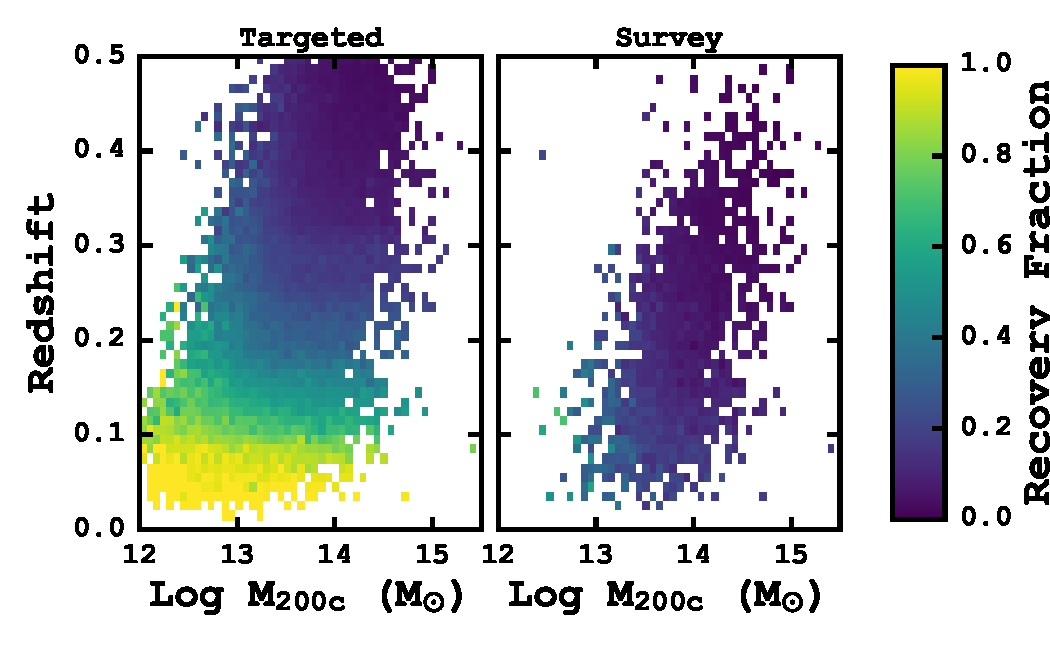
\includegraphics[width=0.8\textwidth]{figures/recovery.pdf} 
	\caption{Recovery fractions ($N_{obs}/N_{True}$) of cluster member galaxies as a function of redshift and true cluster mass for the targeted and survey observing strategies. We have applied HETDEX-like observational limits on the cluster galaxy detection, and require at least five galaxies to be detected for a cluster to be recovered. The solid lines are the median values and the shaded regions represent the 68\% scatter. The significant decline in galaxies observed with the survey strategy is due to gaps in the VIRUS IFU.} \label{fig: recovery} 
\end{figure*}

For the clusters making up the \emph{test} sample the mass is unknown (it is what we are trying to predict) but the other features are known. To determine the mass probability distribution of a test cluster, $P(M)$ we combine the conditional probability distribution, $P(M|\vec{x})$, created previously with the probability distribution of $\sigma$ through Equation~\ref{eq: Pm}.
\begin{equation}\label{eq: Pm}
	P(M) = \int P(M|\vec{x}) P(\sigma) d\sigma
\end{equation}
The expected mass is determined by integrating the mass probability, $P(M)$ over all mass. This becomes our ``predicted'' mass, $\langle M\rangle$.
\begin{equation}\label{eq: expected mass}
	\langle M\rangle = \int M^\prime P(M^\prime)dM^\prime
\end{equation}
The confidence interval associated with this prediction can be estimated two ways. First, by calculating the variance about the expected mass through
\begin{equation}\label{eq: variance}
	\mathrm{Var} = \int (M^\prime - \langle M\rangle)^2 P(M^\prime)dM^\prime
\end{equation}
or by drawing many samples from $P(M)$ and calculating the values at the 16th and 84th percentile. In practice we find that both methods produce similar results for a large number of trials. Therefore, we quote predicted masses as the most probable mass given by Equation~\ref{eq: expected mass} and associated 68\% error estimated through Equation~\ref{eq: variance}.

\subsubsection{Machine Learning Based}\label{sec:machine learning method}
The estimation in this section relies on a ML technique known as an ensemble method, where many estimators are created by a single learning method with the goal of improved generalization and robustness compared to a single estimation. Ensemble methods come in two general flavors. Averaging methods average (hence the name) the estimators to produce a single prediction. Boosting estimators build estimates sequentially by attempting to address poor performing estimators in each previous step, hence ``boosting'' the predictive power.

Here we use an averaging ensemble learning method known as a forest of randomized decision trees often shorten to just random forest (RF). Decision trees can be visualized a flow chart where forks are the branches of the tree. The path along the tree is decided by the values of the feature at each branch. RF estimators use a random subset of the training set at each fork to decide which path should be followed. The final prediction is then the average of all the trees. We use RF regression methods as implemented in {\tt Scikit-Learn} \citep{Pedregosa2012}.

Any uncertainties quoted by this method are prediction intervals not confidence intervals. A prediction interval is an estimate of the interval encompassing future observations, with a certain probability. And, unlike confidence intervals, which describe certainties on the different moments of a population, a prediction interval is unique to each prediction. In many regresson analyses, such as linear fitting, the prediction intervals are based on underlying assumptions of normally distributed residuals. However, RF estimators do not have any such assumptions and require special treatment.

The prediction intervals here are based on the general method of quantile regression forests \citep{Meinshausen2006}. The general idea is that all response variables are recorded, not just the mean. Then the prediction can be returned as the full conditional probability distribution of all responses, which allows us to generate the prediction intervals. The 68\% prediction interval is determined by calculating the 16th and 84th percentile of the full conditional probability distribution. \editorial{I am going to change this to just the std of the distribution. I need the errorbars to be sysmetric to make the fitting routine easy later on.}

\section{RESULTS}\label{sec:results}
Here we explore the cluster member recovery rate and mass estimates for the two observing strategies. We discuss the accuracy of dynamical mass derived from both the scaling relation (see Equation \ref{eq:power law}) and through the probability and ML methods.

\subsection{Recovery of Cluster Members}
As discussed in Section \ref{sec: observations} the observational constraints place limits on the total number fo clusters member galaxies expected to be recovered. Knowing these limits will provide important information for potential future follow up or targeted observations. In this section we discuss the number of cluster members recovered for both the targeted and survey observation strategies, taking into account all observational limits.

Figure \ref{fig: recovery} shows the recovery fraction of member galaxies, the number of observed galaxies divided by the number of actual galaxies ($N_{obs}/N_{True}$), as function of both redshift and cluster mass. It is important to note that if fewer than five member galaxies are observed $N_{obs} <5$ the cluster is not considered detected, and is excluded from this figure. As expected, the targeted observing strategy where the individual clusters are targeted through several dithers to ensure near complete coverage, performs significantly better than the survey observing strategy across all redshifts and cluster masses. 

For the clusters recovered as a function of redshift, there are two effects at work. The decrease in recovery fraction with increasing redshift is a magnitude effect. We check this by limiting the cluster galaxy detection by absolute magnitude which increases the recovery fraction $>70\%$ at all redshifts, implying the decline is a result of the apparent magnitude cluster galaxy detection threshold. The second key feature is the strong decline in clusters recovered from survey observations. This is due to gaps in the VIRUS IFU. The median recovery fraction in survey observations is almost exactly 4.5 times less than the targeted median recovery fraction. As the total filling factor of the survey increases the two lines will converge.

The recovery rate as a function of cluster mass, right panel of Figure \ref{fig: recovery}, shows that of the the low mass clusters we detect ($N_{obs} >5$), we observe the majority of the galaxies. This also shows a rapid decrease in the detection fraction, which can again be explained by considering absolute magnitudes instead of apparent magnitudes, as above. Also, high mass clusters are rare, so inorder to detect them we must probe a large volume of space. The higher redshift cluster members suffer from the limiting apparent magnitude and suppress the recovery fraction at fixed mass. If we were to limit the survey to $z<0.2$ we find the recovery fraction of clusters, at all masses, increases substantially, and we find a much more consistent detection fraction across masses.

\subsection{Mass estimates}
% \begin{table*}
% \centering
% \caption{Summary of the errors associated with the Targeted and Survey observation strategies, as an ensemble of predictions. See the text for discussion about the MAE and RMSE. Overlap is the percentage of clusters where the true cluster mass is bracketed by the prediction intervals of the predicted mass. See Sections \ref{sec:probability method} and \ref{sec:machine learning method} for a discussion on prediction intervals.}
% \begin{tabular}{cccccccc}
% 	%\hline
% 	&& \multic{3}{Targeted} & \multic{3}{Survey} \\
% 	\cline{3-5} \cline{6-8}
% 	& Input Features & MAE & RMSE & Overlap & MAE & RMSE & Overlap \\
% 	& & (dex) & (dex) & (\%) & (dex) & (dex) & (\%) \\
% 	\hline
% 	\rottext{4}{Prob Based} & Power Law & 0.259 & 0.394 & \nd & 0.243 & 0.357 & \nd \\
% 	&$\sigma$ & 0.220 & 0.337 & \nd & 0.210 & 0.310 & \nd \\
% 	&$\sigma, z$ & 0.193 & 0.283 & \nd & 0.184 & 0.271 & \nd \\
% 	&$\sigma, z, N_{gal}$ & 0.128 & 0.204 & \nd & 0.141 & 0.215 & \nd \\
% 	\hline
% 	\rottext{4}{ML Based} & Power Law & 0.258 & 0.394 & \nd & 0.255 & 0.380 & \nd \\
% 	&$\sigma$ & 0.241 & 0.359 & \nd & 0.223 & 0.342 & \nd \\
% 	&$\sigma, z$ & 0.193 & 0.282 & \nd & 0.197 & 0.290 & \nd \\
% 	&$\sigma, z, N_{gal}$ & 0.118 & 0.192 & \nd & 0.140 & 0.221 & \nd \\
% 	\hline
% \end{tabular}
% \label{tbl:mass comparisons}
% \end{table*}

\begin{figure*} 
	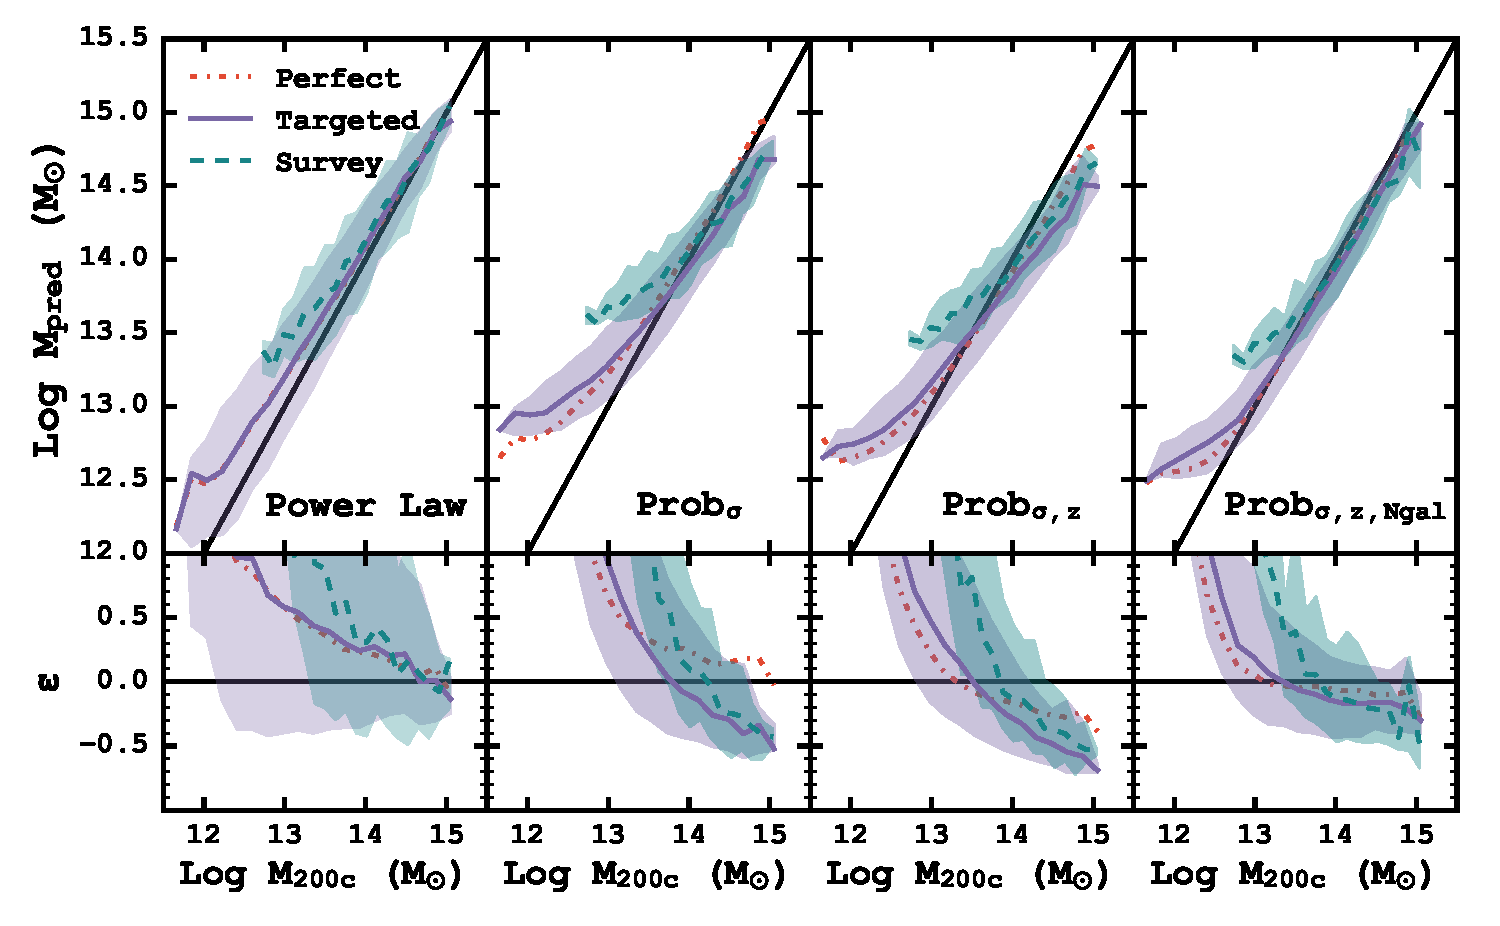
\includegraphics[width=\textwidth]{figures/Probcomparison.pdf} 
	\caption{Mass predictions for the power law scaling relation (Equation~\ref{eq:power law}) and the probability based technique with different input features as a function of true cluster mass. The bottom row of panels shows the fractional error (Equation~\ref{eq: fractional error}) also as a function of true cluster mass. The solid black line shows the 1:1 relation. The solid, colored line is the median predicted mass for the targeted observing, and the colored, dashed line is the median recovered mass for the HETDEX-like observations. The shaded regions represent the 68\% scatter around the median values.} \label{fig:Probability comparison} 
\end{figure*}

In this section we discuss the how accurately we are able to reproduce the true cluster mass from a set of observations. We report on three methods, the power law based approach (Eq. \ref{eq:power law}), the probability based approach (Section \ref{sec:probability method}) and the ML based method (Section \ref{sec:machine learning method}). For each method we consider observations with perfect knowledge, targeted observations and survey observations.

Because it represents the best possible scenario, the perfect knowledge observations should serve as baseline to compare the probability based and ML cluster mass recovery methods. And, while there are many possible metrics to evaluate performance, we compute two: the average bias 
\begin{equation}
\mathrm{\mu_{bias}}(y,\hat{y}) = \frac{1}{N} \sum_{i=0}^N (\hat{y_i} - y_i).\nonumber
\end{equation}
where $y$ is the true value and $\hat{y}$ is the predicted value, and the scatter about the bias
\begin{equation}
	\sigma_{bias}(y,\hat{y}, \mu_{bias}) = \bigg{[}\frac{1}{N-1} \sum_{i=0}^N (\hat{y_i} - y_i - \mu_{bias})^2 \bigg{]}^{1/2}\nonumber
\end{equation}
for different bins of cluster mass. Both metrics evaluate how closely the ensemble of predicted cluster masses are to the true cluster masses, and in both cases values closer to zero are better.

We begin with the perfect knowledge observations. These observations are of the same clusters as the targeted observations but without any observational limits. The cluster masses predicted by Equation \ref{eq:power law} gives the following results. Across all cluster masses, we find $\mu_{bias} = 0.15\pm{0.24}$ dex. The scatter in recovered masses can be attributed to both physical and numerical effects. The presence of any in-falling matter onto lower mass clusters can introduce a significant amount of substructure, which increases the observed LOSVD increasing the predicted mass \citeeg{Ntampaka2015}. Also, as the number of cluster galaxies decreases the LOSVD PDF is poorly sampled leading to poorly recovered cluster masses due to numerical effects. The masses presented here are recovered using the best possible conditions, where we have perfect knowledge of the cluster membership. In reality, the mass recovery levels presented in this section represent an upper bound (the best) on the accuracy achievable through this method.

\editorial{\cite{Ntampaka2015} does have a discussion about how well they do with contaminated galaxy catalogs. We could do something similar and have a similar discussion, but I'm not sure it is worth it. Should be simple enough to do with the targeted catalog, but with the HETDEX catalog it would be pretty bad IMO. We should also talk about how often the true mass lies within the error bars. Many of them are going to be with the 68\% range, but we can drop the error estimates to $0.5\sigma$ if that actually means anything} 

For the targeted and survey observations the power law predicted cluster masses give $\mu_{bias} =0.13\pm{0.37}$ dex and $\mu_{bias} =0.11\pm{0.36}$ dex, respectively. So while, both realistic observations have similar levels of bias, the amount of scatter significantly decreases as more cluster member galaxies are detected, better sampling the LOSVD PDF.

\begin{figure*} 
	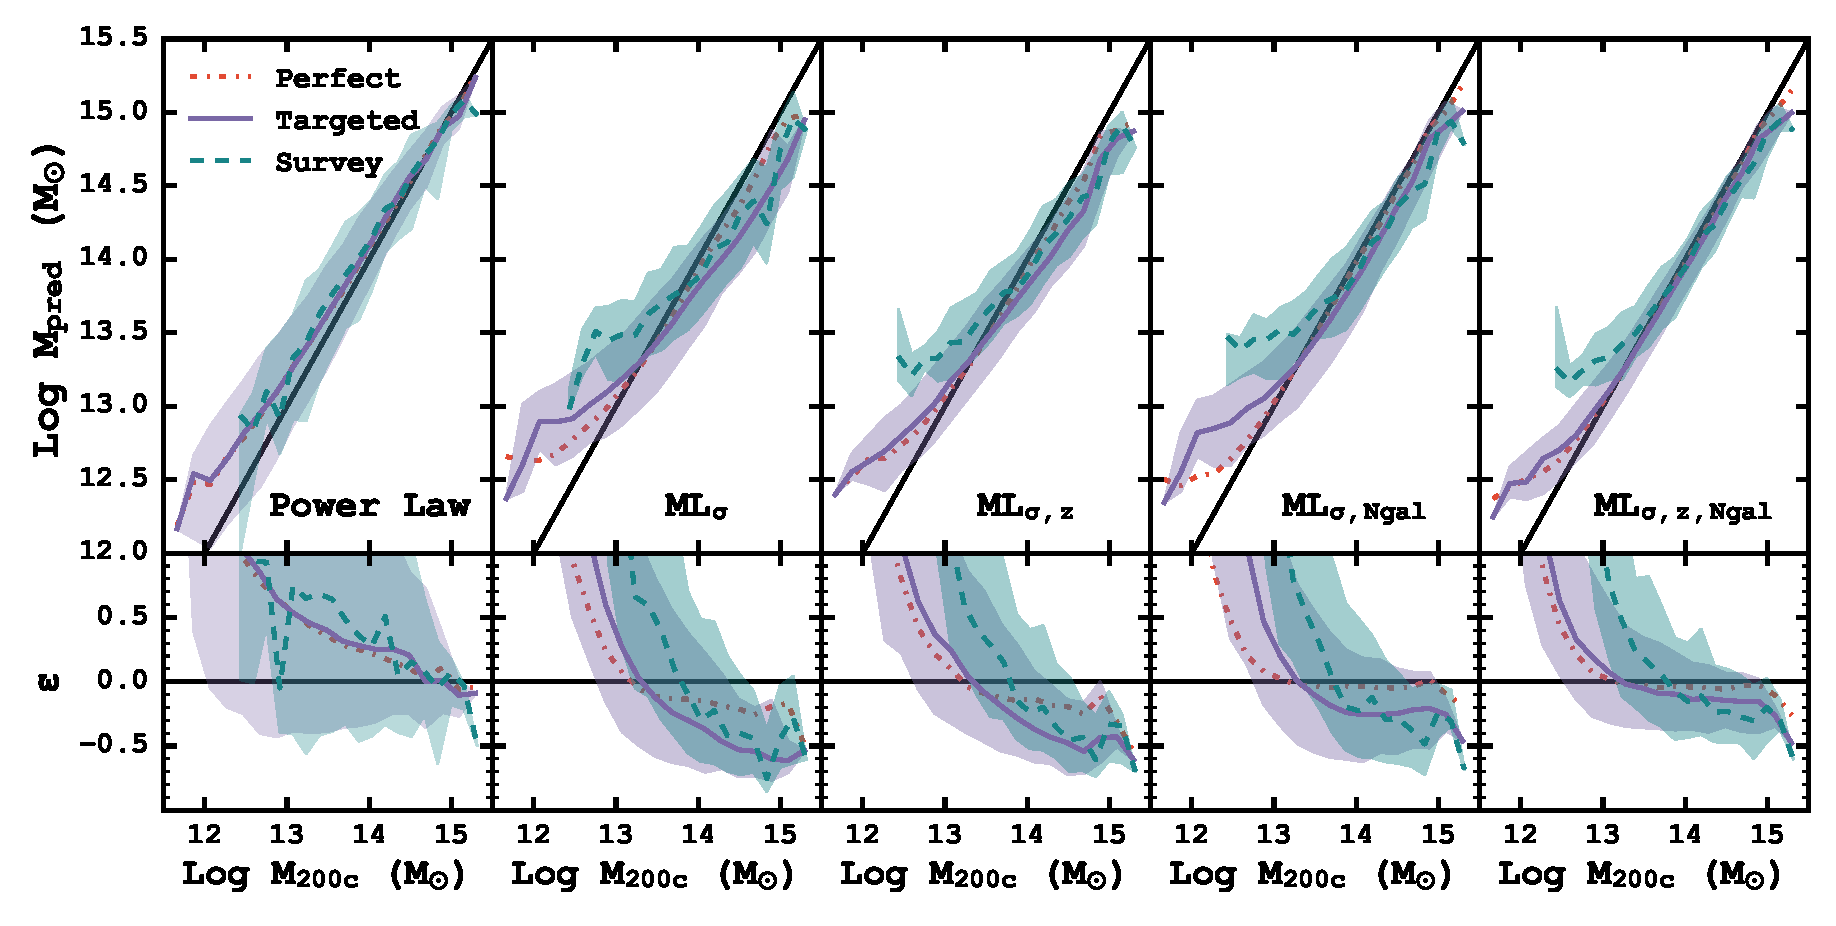
\includegraphics[width=\textwidth]{figures/MLcomparison.pdf} 
	\caption{Mass predictions for the power law scaling relation (Equation~\ref{eq:power law}) and the ML based technique with different input features as a function of true cluster mass. The bottom row of panels shows the fractional error (Equation~\ref{eq: fractional error}) also as a function of true cluster mass. The solid black line shows the 1:1 relation. The solid, colored line is the median predicted mass for the targeted observing, and the colored, dashed line is the median recovered mass for the HETDEX-like observations. The shaded regions represent the 68\% scatter around the median values.} \label{fig: ML comparison} 
\end{figure*}

In both Figures \ref{fig:Probability comparison} and \ref{fig: ML comparison}, we show the predicted versus true cluster masses for each of the two observing strategries. In each panel the solid black line is the 1:1 relationship, the solid purple line is the median recovered mass for the targeted observing, and the turquoise, dashed line is the median recovered mass for the HETDEX-like observations. The shaded regions are the 68\% scatter around the median values (the 16\% and 84\% quartiles). For reference we also show the median masses recovered with perfect knowledge as a solid orange line. The lower panels show the fractional cluster mass error: 
\begin{equation}\label{eq: fractional error}
	\epsilon = (M_{pred} - M)/M
\end{equation}
where $M_{pred}$ is the predicted cluster mass and $M$ is the true cluster mass.

Qualitatively, the top panels of Figures \ref{fig:Probability comparison} and \ref{fig: ML comparison} show that both the probability based and ML based methods out perform (closer to the black 1:1 relation) the power law method when taking advantage of other cluster observables ($z$, $N_{gal}$, etc.). Generally, we find that the single parameter probability and ML methods perform significantly poorer than the power law method, especially at low cluster masses. When combined with the cluster redshift, the predicted cluster masses are improved, even though it is unclear exactly why the additional information should effect the predicted cluster mass. The final addition of the number of observed galaxies, $N_{gal}$ acts as a type of richness estimate, and significantly improves both the bias and the amount of scatter in the predicted masses.


% In both figures we successively add additional information to further constrain the true cluster masses which subsequently reduces the error associated with the ensemble of predictions (see Table \ref{tbl:mass comparisons}). The power law derived masses, using the single (not including the cosmological parameters) free parameter, $\sigma$ (the LOSVD), over estimates the predicted cluster mass at all masses. Both the probability and ML methods over predict the mass of low mass clusters and under predict the mass of the higher mass clusters. When the redshift information is also added, the amount of this over and under prediction is lessened but the cross over point, remains roughly consistent at $\sim10^{14}$ \msol. Additionally, the number of galaxies observed, $N_{gal}$, further reduces the MAE and RMSE on the predictions but also lowers the cross over point to $\sim10^{13.5}$ \msol.

% \editorial{It doesn't look like you can use the targeted training sample to train the survey data. If you do, it either does worse or about the same if you didn't use any training at all. After looking at it, you do have to use the survey training data to get good results about 0.13 dex MAE
% }
\begin{table*}
\centering
\caption{Bias and scatter of the true cluster mass for different bins of predicted cluster mass. This table shows the offset and scatter in the true cluster mass for the perfect (top section), targeted (middle section), and survey (bottom section) observations in different predicted mass bins. The different mass recovery strategies are given in the leftmost column. It can be used to understand how the predicted cluster mass differs from the true cluster masses. Positive numbers indicate the predicted cluster mass over estimates when compared to the true cluster mass.}
\begin{tabular}{cccccccccc} 
		&& \multic{8}{Bins -- Log $M_{pred}$ ($\Msol$)} \\
		\cline{3-10} 
		\multicolumn{2}{c}{Method} & $11.5-12$ & $12-12.5$ & $12.5-13$ & $13-13.5$ & $13.5-14$ & $14-14.5$ & $14.5-15$ & $15-15.5$ \\
		\hline 
		\rottext{4}{Prob Based} & Power Law & $0.49\pm{0.34}$ & $0.28\pm{0.39}$ & $0.23\pm{0.34}$ & $0.16\pm{0.22}$ & $0.11\pm{0.16}$ & $0.07\pm{0.14}$ & $0.02\pm{0.14}$ & $-0.07\pm{0.10}$ \\
		&$\sigma$ & $0.87\pm{0.15}$ & $0.53\pm{0.24}$ & $0.32\pm{0.26}$ & $0.16\pm{0.20}$ & $0.10\pm{0.16}$ & $0.07\pm{0.14}$ & $0.05\pm{0.16}$ & $-0.18\pm{0.17}$ \\
		&$\sigma, z$ & $0.76\pm{0.16}$ & $0.42\pm{0.21}$ & $0.17\pm{0.23}$ & $0.01\pm{0.19}$ & $-0.06\pm{0.16}$ & $-0.11\pm{0.55}$ & $-0.14\pm{0.16}$ & $-0.38\pm{0.34}$ \\
		&$\sigma, z, N_{gal}$ & $0.65\pm{0.10}$ & $0.28\pm{0.14}$ & $0.04\pm{0.47}$ & $-0.02\pm{0.14}$ & $-0.02\pm{0.10}$ & $-0.05\pm{0.54}$ & $-0.22\pm{1.61}$ & $-6.62\pm{8.08}$ \\
		\hline
		\rottext{4}{ML Based} & Power Law & $0.49\pm{0.34}$ & $0.28\pm{0.39}$ & $0.23\pm{0.34}$ & $0.16\pm{0.22}$ & $0.11\pm{0.16}$ & $0.07\pm{0.14}$ & $0.02\pm{0.14}$ & $-0.07\pm{0.10}$ \\
		&$\sigma$ & $0.69\pm{0.20}$ & $0.36\pm{0.27}$ & $0.15\pm{0.29}$ & $-0.02\pm{0.24}$ & $-0.07\pm{0.21}$ & $-0.09\pm{0.19}$ & $-0.11\pm{0.18}$ & $-0.12\pm{0.19}$ \\
		&$\sigma, z$ & $0.62\pm{0.18}$ & $0.33\pm{0.22}$ & $0.12\pm{0.25}$ & $-0.01\pm{0.20}$ & $-0.06\pm{0.18}$ & $-0.09\pm{0.16}$ & $-0.11\pm{0.17}$ & $-0.19\pm{0.13}$ \\
		&$\sigma, z, N_{gal}$ & $0.51\pm{0.14}$ & $0.23\pm{0.18}$ & $0.05\pm{0.17}$ & $-0.02\pm{0.14}$ & $-0.02\pm{0.10}$ & $-0.02\pm{0.08}$ & $-0.02\pm{0.08}$ & $-0.08\pm{0.08}$ \\
		\hline 
		\hline
		\rottext{4}{Prob Based} & Power Law & $0.49\pm{0.31}$ & $0.27\pm{0.41}$ & $0.20\pm{0.43}$ & $0.13\pm{0.39}$ & $0.10\pm{0.33}$ & $0.09\pm{0.27}$ & $0.02\pm{0.18}$ & $-0.08\pm{0.09}$ \\
		&$\sigma$ & $1.02\pm{0.13}$ & $0.66\pm{0.19}$ & $0.40\pm{0.24}$ & $0.17\pm{0.25}$ & $0.02\pm{0.25}$ & $-0.08\pm{0.22}$ & $-0.19\pm{0.19}$ & $-0.35\pm{0.26}$ \\
		&$\sigma, z$ & $0.85\pm{0.18}$ & $0.49\pm{0.20}$ & $0.25\pm{0.24}$ & $0.08\pm{0.24}$ & $-0.06\pm{0.23}$ & $-0.21\pm{0.56}$ & $-0.35\pm{0.21}$ & $-0.59\pm{0.31}$ \\
		&$\sigma, z, N_{gal}$ & $0.70\pm{0.13}$ & $0.37\pm{0.18}$ & $0.13\pm{0.20}$ & $0.01\pm{0.19}$ & $-0.05\pm{0.17}$ & $-0.12\pm{0.67}$ & $-0.44\pm{2.26}$ & $-4.45\pm{7.44}$ \\
		\hline
		\rottext{4}{ML Based} & Power Law & $0.49\pm{0.31}$ & $0.27\pm{0.41}$ & $0.20\pm{0.43}$ & $0.13\pm{0.39}$ & $0.10\pm{0.33}$ & $0.09\pm{0.27}$ & $0.02\pm{0.18}$ & $-0.08\pm{0.09}$ \\
		&$\sigma$ & $0.76\pm{0.28}$ & $0.54\pm{0.29}$ & $0.26\pm{0.31}$ & $0.01\pm{0.31}$ & $-0.13\pm{0.32}$ & $-0.23\pm{0.30}$ & $-0.33\pm{0.29}$ & $-0.32\pm{0.09}$ \\
		&$\sigma, z$ & $0.66\pm{0.13}$ & $0.37\pm{0.23}$ & $0.17\pm{0.26}$ & $0.03\pm{0.25}$ & $-0.09\pm{0.24}$ & $-0.21\pm{0.22}$ & $-0.31\pm{0.25}$ & $-0.28\pm{0.13}$ \\
		&$\sigma, z, N_{gal}$ & $0.57\pm{0.12}$ & $0.28\pm{0.21}$ & $0.09\pm{0.21}$ & $-0.01\pm{0.18}$ & $-0.05\pm{0.16}$ & $-0.08\pm{0.14}$ & $-0.07\pm{0.12}$ & $-0.14\pm{0.13}$ \\
		\hline
		\hline
		\rottext{4}{Prob Based} & Power Law & \nd & \nd & $0.53\pm{0.15}$ & $0.30\pm{0.29}$ & $0.16\pm{0.33}$ & $0.07\pm{0.31}$ & $0.01\pm{0.24}$ & $-0.09\pm{0.13}$ \\
		&$\sigma$ & \nd & \nd & $0.77\pm{0.10}$ & $0.42\pm{0.18}$ & $0.18\pm{0.22}$ & $-0.03\pm{0.22}$ & $-0.18\pm{0.19}$ & $-0.39\pm{0.22}$ \\
		&$\sigma, z$ & \nd & \nd & $0.61\pm{0.12}$ & $0.29\pm{0.19}$ & $0.08\pm{0.22}$ & $-0.11\pm{0.21}$ & $-0.38\pm{1.30}$ & $-0.48\pm{0.27}$ \\
		&$\sigma, z, N_{gal}$ & \nd & \nd & $0.48\pm{0.13}$ & $0.18\pm{0.18}$ & $0.02\pm{0.19}$ & $-0.08\pm{0.19}$ & $-0.50\pm{2.25}$ & $-8.81\pm{7.98}$ \\
		\hline
		\rottext{4}{ML Based} & Power Law & \nd & $0.06\pm{0.80}$ & $0.17\pm{0.39}$ & $0.17\pm{0.41}$ & $0.13\pm{0.38}$ & $0.07\pm{0.32}$ & $0.01\pm{0.24}$ & $-0.09\pm{0.13}$ \\
		&$\sigma$ & \nd & $0.58\pm{0.17}$ & $0.54\pm{0.26}$ & $0.24\pm{0.28}$ & $0.03\pm{0.30}$ & $-0.17\pm{0.30}$ & $-0.26\pm{0.30}$ & $-0.30\pm{0.25}$ \\
		&$\sigma, z$ & \nd & $1.02\pm{0.35}$ & $0.42\pm{0.21}$ & $0.19\pm{0.25}$ & $0.03\pm{0.25}$ & $-0.14\pm{0.25}$ & $-0.25\pm{0.24}$ & $-0.31\pm{0.26}$ \\
		&$\sigma, z, N_{gal}$ & \nd & $0.91\pm{0.45}$ & $0.39\pm{0.19}$ & $0.12\pm{0.21}$ & $-0.00\pm{0.20}$ & $-0.08\pm{0.19}$ & $-0.14\pm{0.19}$ & $-0.21\pm{0.20}$ \\
	\hline
	\end{tabular}
\label{tbl:mass bias}
\end{table*}

We quantify the bias and scatter for all of the different cluster mass recovery strategies and observing methods in Table \ref{tbl:mass bias}. It should serve as a type of look up table for future cluster observations with HETDEX. The columns represent bins of predicted galaxy cluster mass and the individual values show the bias and scatter of the true cluster mass. The three horizontal sections represent represent perfect, targeted and survey observations respectively. So, for example, if a cluster mass is predicted using the $ML_{\sigma, z}$ method and targeted observations to be Log M $=13-13.5$ \Msol, it is biased upward by $0.03\pm0.25$ dex. 

 A few caveats apply to the numbers given in Table \ref{tbl:mass bias}. While we provide corrections for cluster masses above $10^{15}$, they are estimated from only a handful of objects, and do not constitute a representative sample of clusters. On the oposite end of the cluster mass spectrum, survey observations of low mass clusters are incomplete for two potential reasons. There are very few, if any, clusters detected with survey observations below $10^{12}$. Missing corrections above $10^{12}$ in the probability based methods are due to low number statstics and an inability to sample the cluster mass PDF well enough to assign cluster mass predictions.




\section{HETDEX as a Galaxy Cluster Survey at $z < 0.5$}\label{sec:discussion}



\subsection{Extendability to Other Surveys}
Large-scale optical surveys (\eg, DES and LSST) expect to detect hundreds of thousands of galaxy clusters at $z < 1$. Because they are photometric, a major challenge for these surveys is relating a cluster observable to the total dark-matter mass. One promising mass estimator is the optical richness \citeeg{Abell1958}. Specifically, here, we use $\lambda$, the weighted number of galaxies within a scale aperture \citeeg{Rozo2011} as calculated by the redMapper algorithm \citep{Rykoff2012}. Previous works \citeeg{Rozo2010} show that the richness correlates strongly with cluster mass on the average, but the absolute mass scale of the optical richness mass estimator and the scatter in cluster mass at fixed optical richness are imprecisely known \citep{Rykoff2012}. These systematics remain the major source of uncertainty in deriving cosmological constraints from cluster abundances and must be measured using independent methods to realize the full potential of these surveys.

\begin{figure} 
	\includegraphics[width=\columnwidth]{figures/massRichness_targeted.pdf} 
	\caption{The optical richness, $\lambda$, versus the predicted cluster mass. The purple and blue points represent clusters with targeted and survey detections respectively. Error bars show $1\sigma$ prediction interval. The solid and dashed lines are fits to either the targeted or survey sets. } \label{fig:mass richness} 
\end{figure}

We leverage the large spectroscopic dataset of HETDEX to estimate its ability to constrain the scatter and absolute scale of the richness-mass relationship. We begin by cross matching both the targeted and survey observations with a redMapper catalog. The redMapper catalog is limited to $\lambda >= 20$, or at least twenty object assigned to each cluster. With the targeted and survey observations, we observe 138 and 58 clusters respectively. 

Figure \ref{fig:mass richness} shows the optical richness, $\lambda$, versus the predicted cluster mass. The cluster masses are the $ML_{\sigma, z, N_{gal}}$ based and correspond to the correct observation strategy. The error bars represent the $1\sigma$ prediction intervals for each cluster mass. The solid and dashed lines are fits to the targeted and survey datasets. For comparison, the richness-mass relations from \cite{Rykoff2012} (their equation B5) is shown as a dash-dotted line.

To generate the best fitting lines we follow the general procedure of \cite{Hogg2010}, by defining an objective function and then minimizing the loss. Our loss function is
\begin{equation}
	\mathrm{ln}L= \frac{-1}{2} \bigg{(} \sum^N_{i=1}\frac{[y_i - mx_i - b]^2}{\sigma_{yi}} + \sum^N_{i=1}\frac{[y_i - mx_i - b]^2}{\sigma_{xi}} \bigg{)}
\end{equation} 
where we have taken into account the uncertainties in both the richness and predicted cluster mass. We again rely on MCMC samples to sample the posterior probability distribution. The best fitting slope and intercept are quoted as the median value of the posterior probability distribution with 68\% error bars defined as the 16th and 84th percentiles of the same distribution.

Following the notation of \cite{Rykoff2012} we find a best-fitting relation for the targeted observations as
\begin{equation}
	ln\bigg{(}\frac{M_{200c}}{h_{70}^{-1} 10^{14}\Msol}\bigg{)} = 1\pm0.13 + 1.34\pm0.17 ln\bigg{(}\frac{\lambda}{60}\bigg{)} \nonumber
\end{equation}
and the survey observations as
\begin{equation}
	ln\bigg{(}\frac{M_{200c}}{h_{70}^{-1} 10^{14}\Msol}\bigg{)} = 1.02\pm0.13 + 0.96\pm0.22 ln\bigg{(}\frac{\lambda}{60}\bigg{)} \nonumber
\end{equation}

The bottom panel of Figure \ref{fig:mass richness} shows the scatter in cluster masses at fixed richness, $\sigma_{M|\lambda}$. The solid and dashed lines represent the targeted and survey observations respectively, and have been offset from one another for clarity. The cluster masses are binned in increasing ten richness intervals ($20-30$, $30-40$, etc.). The two horizontal lines show the mean scatter of 0.26 dex for the targeted observations and 0.21 dex for the survey observations. While not shown in the figure, we find a mean scatter of 0.27 dex if we replace $M_{pred}$ with the true cluster mass for the clusters identified with targeted observations. The reduction in scatter from the targeted to survey observations is due to fewer objects detected in survey mode.

%Much like the MAE and RMSE associated with the cluster mass recovery, comparing the individual $\sigma_{M|\lambda}$ values directly is incorrect. When comparing only the clusters with observations in both the targeted and survey strategies we 
	
%Applying my current work to a large photometric survey such as those mentioned above is the logical next step. For example, the HETDEX observations overlap with the DES area and SDSS Stripe 82 which provides a wealth of external data. Using preexisting datasets, the observations from HETDEX, or through dedicated followup spectroscopic observations, I will be able to measure the absolute mass scale of the richness estimator and measure the scatter of the richness-mass relation, $\sigma_{M|\lambda}$. An accurate measure of this scatter can lead to a decrease on the error bar on cosmological measures ($\sigma_8$ and $\Omega_M$) by as much as 50\% \citep{Rozo2010}. An absolute calibration of the richness-mass relation will provide a much needed tool for future imaging surveys which will identify clusters to $z=1$ and beyond.

\subsection{Potential Improvements}
\editorial{The potential improvements are really three fold. We know that the observing won't cover all of the sky. So we can simply tile more and try to get more clusters. We can observe deeper. I'm not sure the current exposure times (they are in an email that I sent to casey) but if we can extend them, then we can get further down the IMF and try to build up some of the clusters that are really more like groups than anything else. The last thing we can do is to attempt to  build better models to make better predictions on the masses. That might be something like the study that \cite{Acquaviva2016} did with the stellar metallicities. Or we'll need something else that I haven't thought of just yet. The other idea is to come up with some sort of cheat sheet for HETDEX. Basically, a if you detect such and such type of galaxy in the survey model then you should go back and try to follow it up with targeted observations. It might be good to talk about the recovery fraction between the two surveys above. Like... if there are 30 cluster members then we should detect the cluster in both surveys.}

\section{SUMMARY}\label{sec:summary}
Here, we present detailed simulations of the upcoming HETDEX survey's applicability to the detection and total mass measurement of galaxy clusters. We use mock galaxy catalogs, and simulated HETDEX-like observational strategies to estimate the number of clusters observed and the precision of their total mass estimates, using three different mass estimates. With an eye to galaxy cluster studies, we discuss potential improvements to the HETDEX survey, and comment on how HETDEX may improve current and future photometric large-area sky surveys' cluster mass estimates derived from optical richness.

Our main conclusions are the following:
\begin{enumerate}
	\item HETDEX-like observations do a good job observing galaxy clusters. The number of galaxy clusters detected in the HETDEX-like observations is almost exact 4.5 times less than in the targeted observations. This difference is the same as the overall HETDEX fill factor.
	\item Overall, we find that a traditional power-law conversion from LOSVD to cluster mass performs significantly poorer than either the probability based or ML based methods also tested. We find the MAE and RMSE of survey detected cluster mass estimates to be approximately 38\% and 65\% respectively, compared to approximately 123\% when a power-law is used alone.
	\item While the power-law may be outperformed, overall, comparisons of similar mass galaxy clusters shows that above Log M $=14.5$ \Msol, the power-law gives a lower MAE than either the probability based or ML based methods. For HETDEX-like observations and clusters with $13 < Log M <14.5$ \Msol, we find the $ML_{\sigma, z, N_{gal}}$ method performs the best. Below Log M $=13$ \Msol\ no method with survey observations gives an MAE of less than 50\%.
	\item For followup targeted observations only galaxy clusters with masses inferred to be Log M $<13$ \Msol\ from survey observations should be targeted. Galaxy clusters with inferred masses below Log M $=13$ \Msol\ can see as much as an 81\% improvement in cluster mass estimation with targeted observations. While the improvement of clusters with masses above Log M $=13$ \Msol\ is often approximately 10\%.
	\item \editorial{Something about the richness.}
\end{enumerate}

It is the author's hope that this work may be useful to others when conducting their own research. Because this work relies heavily on (often) complex data analysis, and in order to promote transparency and reproducible science, we provide all of the code used to conduct this study at https://github.com/boada/desCluster. Regrettably, large file size prevents including the source data with the analysis routines. The authors are happy to provide them, if requested.

\section*{Acknowledgements}
The authors also wish to thank the anonymous referee whose comments and suggestions significantly improved both the quality and clarity of this work. We also thank Steven W. Crawford for many helpful discussions. This research made use of This research made use of  the {\tt IPython} package \citep{Perez2007} and {\tt matplotlib}, a Python library for publication quality graphics \citep{Hunter2007}. Figure \ref{fig: probability corner} is heavily based on \cite{Foreman-Mackey2016}. Funding for the SDSS and SDSS-II has been provided by the Alfred P. Sloan Foundation, the Participating Institutions, the National Science Foundation, the U.S. Department of Energy, the National Aeronautics and Space Administration, the Japanese Monbukagakusho, the Max Planck Society, and the Higher Education Funding Council for England. The SDSS Web Site is http://www.sdss.org/. The SDSS is managed by the Astrophysical Research Consortium for the Participating Institutions. \editorial{People to thank: Joe, maybe authorship.}

%%%%%%%%%%%%%%%%%%%% REFERENCES %%%%%%%%%%%%%%%%%%
% The best way to enter references is to use BibTeX:
\bibliographystyle{mnras}
\bibliography{master} % if your bibtex file is called example.bib

%%%%%%%%%%%%%%%%% APPENDICES %%%%%%%%%%%%%%%%%%%%%
% \appendix
%
% \section{Some extra material}
%
% If you want to present additional material which would interrupt the flow of the main paper,
% it can be placed in an Appendix which appears after the list of references.

% Don't change these lines
\bsp	% typesetting comment
\label{lastpage}
\end{document}

% \begin{equation}
%     x=\frac{-b\pm\sqrt{b^2-4ac}}{2a}.
% 	\label{eq:quadratic}
% \end{equation}
%
% % Example figure
% \begin{figure}
% 	% To include a figure from a file named example.*
% 	% Allowable file formats are eps or ps if compiling using latex
% 	% or pdf, png, jpg if compiling using pdflatex
% 	\includegraphics[width=\columnwidth]{example}
%     \caption{This is an example figure. Captions appear below each figure.
% 	Give enough detail for the reader to understand what they're looking at,
% 	but leave detailed discussion to the main body of the text.}
%     \label{fig:example_figure}
% \end{figure}
%
% % Example table
% \begin{table}
% 	\centering
% 	\caption{This is an example table. Captions appear above each table.
% 	Remember to define the quantities, symbols and units used.}
% 	\label{tab:example_table}
% 	\begin{tabular}{lccr} % four columns, alignment for each
% 		\hline
% 		A & B & C & D\\
% 		\hline
% 		1 & 2 & 3 & 4\\
% 		2 & 4 & 6 & 8\\
% 		3 & 5 & 7 & 9\\
% 		\hline
% 	\end{tabular}
% \end{table}

% \section{Evidence of Substructure}
% Like the recovery of dynamical parameters discussed in the previous section, the choice of method to investigate the dynamical state of galaxy clusters is heavily debated. Perhaps the most widely used metric is the Dressler-Shectman (DS) test \citep{Dressler1988}, and is not without criticism \citeeg{White2010}. New methods such as the Caustic Method (\citealt{Yu2015}, and the references therein) offer promise to shed further light on this difficult problem.
%
% \subsection{From VD profiles}
% We utilize the modality \citep{Oliva-Altamirano2014} which describes the Gaussianity of a LOSV distribution in a galaxy cluster. For clusters with Gaussian distributed LOSVs, the modality is close to 1/3. It is defined as $(1+\mathrm{skewness}^2)/(3+\mathrm{kurtosis}^2)$. \editorial{Do I need to describe what the skewness and kurtosis is?}
%
% \subsection{Dominance}
% \editorial{This is taken pretty directly from the GAMA paper. Will need to be edited to fit.}
% The dominance is defined as the luminosity gap between the brightest and the second brightest galaxy in a cluster ($\Delta m_{1, 2}$). The amplitude of the luminosity gap between the BGG/BCG and the second brightest galaxy in the halo, is expected to be a function of both the formation epoch and the recent infall history of the halo. A small magnitude gap ($\Delta m_{1, 2} < 1$) indicates a recent halo merger, and larger gaps ($\Delta m_{1, 2} > 1$), common in fossil groups, is perhaps indicative of a cluster or groups that has not undergone a recent merger.
%
% \subsection{Dressler-Schectman Test}
% We leverage the large spectroscopic dataset to study the structural properties of the clusters. \cite{Pinkney1996} determine, from a comparison of five different methods that the DS test is the most sensitive to the presence of substructure.
%
% The DS test, which combines the spatial positions and velocities of the galaxies, provides a method to locate substructure by identifying groups of galaxies which differ significantly from the cluster velocity distribution. Galaxy subsets are selected from a cluster of $n_{members}$ and each constituent galaxy deviation is calculated according to
% \begin{equation}
% 	\delta_i^2 = \frac{N_{local}+1}{\sigma^2}\bigg{[}(\bar{v}_{local,i} - \bar{v})^2 + (\sigma_{local,i} - \sigma)^2\bigg{]}^2
% \end{equation}
% where $\bar{v}_{local}$ and $\sigma_{local}$ are the mean velocity and velocity dispersion for a subset of $N_{local}$ galaxies and $\bar{v}$ and $\sigma$ are the entire cluster's mean velocity and velocity dispersion. The choice of $N_{local}$ is left to the user. Originally, \cite{Dressler1988} choose $N_{local}=10$, however \cite{Bird1994} points out that using a fixed value for $N_{local}$ reduces the sensitivity to substructure. We follow \cite{Bird1994} in choosing $N_{local} = \sqrt n_{members}$. \editorial{doesn't talk about the nearest neighbors which is what we are using.}
%
% The DS statistic is the $\Delta$-value given by,
% \begin{equation}
% 	\Delta = \sum^{n_{members}}_i \delta_i
% \end{equation}
% where a system is considered to contain substructure if $\Delta/n_{members} > 1$ \citep{Dressler1988}. A second method, described in \cite{Hou2012}, uses probabilities (P-values) rather than a threshold for the identification of substructure. P-values are computed by comparing the observed $\Delta$-value and the $Delta$-value after the velocities (but not positions) have been shuffled through a series of Monte Carlo runs. The probability of the existence of substructure becomes
% \begin{equation}
% 	P = \sum (\Delta_{shuffled} > \Delta_{Observed}) / n_{shuffle}
% \end{equation}
% where $n_{shuffle}$ is the number of shufflings used. \editorial{This sounds a whole lot like the description given in Hou2012. Make sure that we aren't copying anything word for word. That'd be bad.}
%
% In practice, we use locate the nearest neighbors using an unsupervised k-nearest neighbor algorithm as implemented in Scikit-Learn \citep{Pedregosa2012}.
